In the last few decades we are witnessing a fast and numerous shift from dedicated single object observations to massive all-sky surveys producing hundreds or even thousands of unbiased observations in a single telescope pointing. Along with the complexity of data acquisition and storage, new challenges and problems involving data reduction arose, requiring dedicated computer power to reduce acquired data. The reduction challenges span from timely, almost real-time reduction requirements, to complex, computationally demanding processes that try to take into account as many telescopically and observationally induced biases as possible. Some of those processes will be discussed in the following sections discussing a specific survey.

This thesis shows few cases of synergies of such vastly different data sets and at the same time points to a necessity of having knowledge about the automatic processing pipelines that produced final products, quite often blindly used by users.

The main source of data for our studies are the following three stellar surveys producing informations about the stars' brightness, composition, distance, kinematics and many additional parameters that can be inferred from the observed quantities.

\begin{figure}
	\centering
	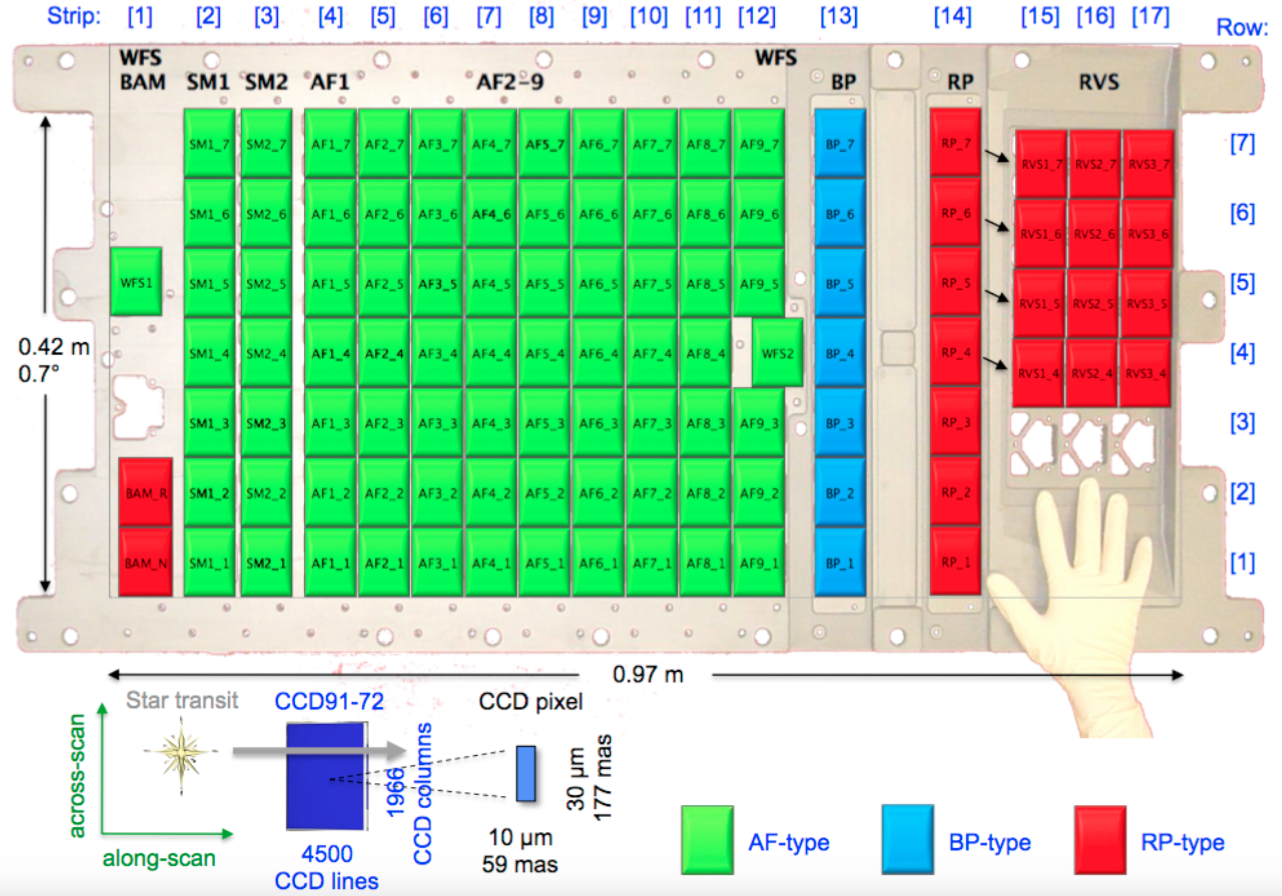
\includegraphics[width=\columnwidth]{gaia_ccd.png}
	\caption{Size comparison and spatial arrangement of the CCD detectors in the Gaia focal plane. Image credit: \citet{2016A&A...595A...1G}.}
	\label{fig:gaia_ccd}
\end{figure}

\section{Gaia}
\label{sec:gaia_data}
Gaia is the one-billion-star surveyor of the European Space Agency (ESA). It has been continuously scanning the sky since July 2014 from its designated location close to the second Lagrange point of the Sun-Earth/Moon system. Gaia’s aim is to map the entire sky,down to magnitude $\sim20.7$, and to collect micro-arcsecond-level astrometry and milli-magnitude-level photometry for the brightest 1,000+ million stars as well as medium-resolution spectroscopy for mainly radial-velocity determination of the brightest subset of $\sim150$ million objects. 

The Gaia scanning of the sky is composed of two independent, superimposed motions: a rotation around the spacecraft spin axis with a period of 6 hours plus a slow, 63 day period precession of the spin axis around the Solar direction at a fixed Solar-aspect angle of $45^\circ$. Over the nominal five-
year mission, Gaia has completed $29$ of these precession periods, leading to an optimally uniform sky coverage with, on average, $\sim70$ astrometric and photometric transits across the focal plane (and $\sim40$ for the spectroscopic instrument). In the extended mission phase that started in July 2019, a similar scanning law is being employed but with a reversed precession direction during the first year. A passage of a star through the focal plane is called a field-of-view transit. During each transit, Gaia collects instantaneous, so-called epoch data of each object. Publication of all epoch data is scheduled (see Table \ref{tab:gaia_drs} for the final data release.

\begin{table}
	\centering
	\caption{Past and future predicted release dates of Gaia data and products.}
	\begin{tabular}{c c}
		\hline
		Release designation & Date \\ 
		\hline
		Gaia DR1 & 14 September 2016 \\
		Gaia DR2 & 25 April 2018 \\
		Gaia EDR3 & 3$^{rd}$ quarter of 2020 \\
		Gaia DR3 & 2$^{nd}$ half of 2021 \\
		Final release & not yet determined \\
		\hline
	\end{tabular}
	\label{tab:gaia_drs}
\end{table}

As the spacecraft slowly rotates, observed stars traverse the Gaia focal plane equipped with 106 CCD detectors (show in Figure \ref{fig:gaia_ccd}). Every star that gets observed therefore passes trough a sequence of those detectors who analyse a star in the given order:

\subsection{Photometry and astrometry}
The first array of CCDs that collects light from stars is a Sky Mapper (SM) that autonomously detect objects. Stars brighter than magnitude $\sim3$ are too bright to be detected automatically. The faint detection threshold is set at $20.7$ magnitude in the Gaia G band but is not infinitely sharp due
to on-the-fly magnitude estimation errors of the on-board software.

After the source detection, stars pass into the largest array of CCDs that is attributed to the Astrometric Field (AF). It collects the instantaneous positions and fluxes of all objects detected by the Sky Mapper as they traverse along the field. Astrometric measurements are made in a white-light bandpass, covering the range from 3300 to 10500 \AA, which is referred to as the Gaia G band.

The last spectro-photometric measurements are thereafter performed by two low dispersion detectors that are measuring precise fluxes in a number of narrow-pass sub-bands of previously mentioned wide-pass G band. The Blue Photometer (BP) collects low resolution spectra of all objects over the wavelength range from 3300 to 6800 \AA. The integrated magnitude is referred to as the G$_{BP}$ or BP magnitude. The Red Photometer (RP) collects low-resolution spectra of all objects over the wavelength range from 6300 to 10500 \AA. The integrated magnitude is referred to as the G$_{RP}$ or RP magnitude.

\subsection{Spectroscopy}
A final measurement performed by the spacecraft is spectroscopy over the whole observed field of the sky. The integral-field Radial Velocity Spectrometer (RVS) \citep{2018A&A...616A...5C} collects medium-resolution spectra (spectral resolving power (R) $\sim11,700$) over the wavelength range from 8450 to 8720 \AA, for all objects brighter than magnitude $\sim16$ in this bandpass. The location of the pass-band is selected to cover the ionised calcium (CaII) triplet with a prominent absorption features over a large temperature range of stars and can therefore be used to determine radial velocity of spectrally diverse stars. The integrated magnitude in the RVS bandpass is referred to as the G$_{RVS}$ magnitude. The RVS has a reduced field of view orthogonal to the scan direction such that fewer observations up to the RVS limiting magnitude are collected compared to photometric fields in a ratio of 4:7.

\section{Gaia DR2}
\label{sec:gaia_dr2_data}
The second data release of Gaia data (Gaia DR2) was heavily used during the production of this thesis, therefore it requires detailed description of provided tables, its use and potential problems. The release set is far from complete and similar to the final release, but on the other hand provides an unprecedented set of homogeneously acquired and reduced stellar informations newer seen before. Visual and numerical representation of the specific stellar product is given in Figure \ref{fig:gaia_drs}. Gaia DR2 is based on data collected by the spacecraft between 25 July 2014 and 23 May 2016, spanning a period of 22 months. 

\begin{figure}
	\centering
	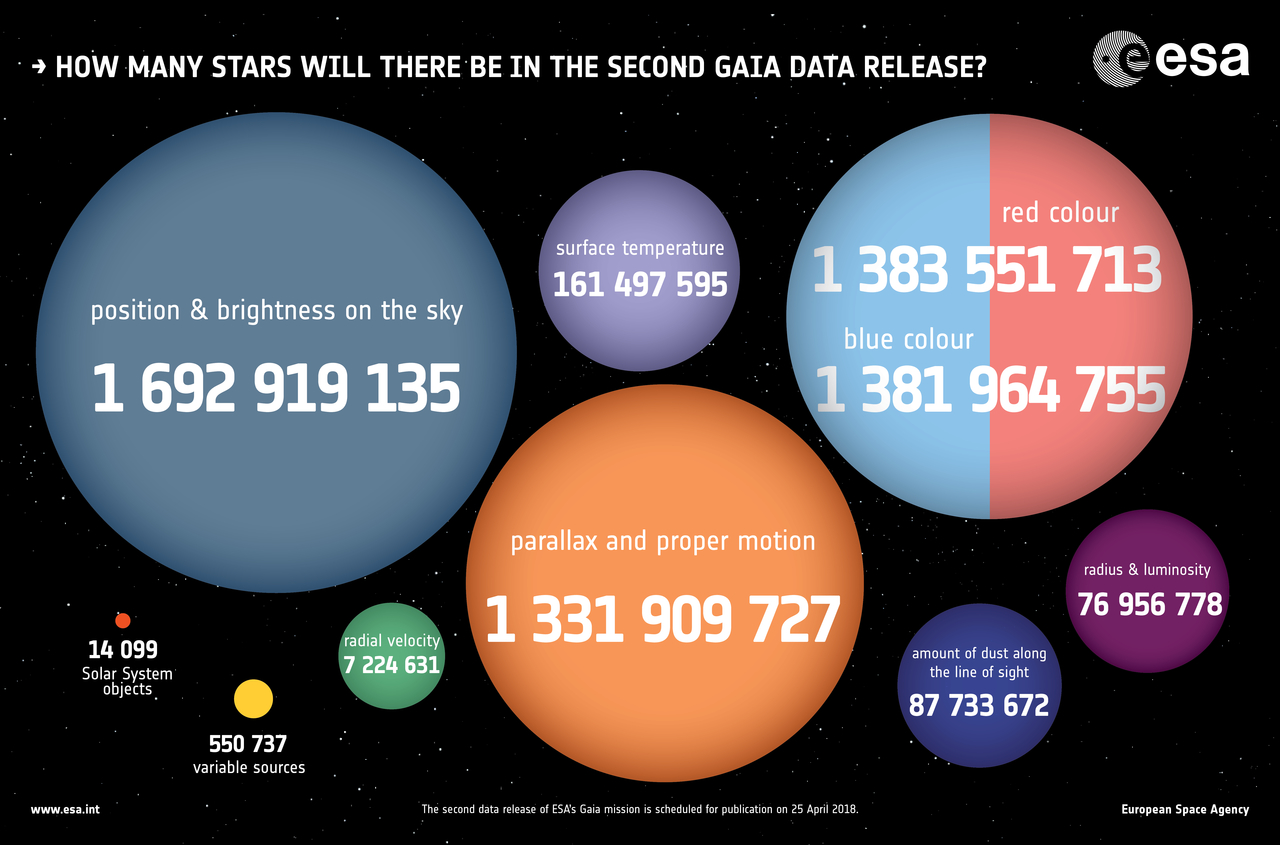
\includegraphics[width=\columnwidth]{1567214817936-Gaia_DR2_numbers_1280.jpg}
	\caption{Visual and numerical representation of Gaia DR2 stellar content. Image credit: ESA, CC BY-SA 3.0 IGO.}
	\label{fig:gaia_drs}
\end{figure}

Along the calibrated raw measurements, Gaia Data Processing and Analysis Consortium (DPAC) provides numerous parameters and properties of stars, pre-selected Solar system bodies and quasars that can be used and explored by users. Among them we can find:
\begin{itemize}
	\item \textbf{Astrometric set} consisting of partial 2-parameter (limited to celestial positions $\alpha$ and $\delta$) and full 5-parameter astrometric solution with addition of including parallax, and proper motion. The 2-parameter sources are typically faint (with about half of them at magnitude G > 20.6), have very few observations (less than five as required for full solution), or very poorly fit the five-parameter astrometric model. All sources fainter than magnitude G = 21 have only positional information. In the current data release all stars are still treated as single during astrometric fit, which could significantly influence solutions in the case of multiple fast moving sources contributing to the position of an observed photocentre. The Gaia coordinate reference frame is aligned with the International Celestial Reference Frame (ICRF) using positions of extragalactic sources such as quasars \citep{2018A&A...616A..14G}. After the initial release, it was determined that the quality of an astrometric fit is best described by the renormalised astrometric chi-square (RUWE) \citep{ruwe}. Further details about astrometric processing and validation are given in \citet{2018A&A...616A...2L, 2018A&A...616A...9L}.
	
	\item \textbf{Photometric data set} contains the broad band photometry in the G, G$_{BP}$, and G$_{RP}$ bands, giving us colour information for Gaia DR2 sources that were observed at least twice. The mean value of the G-band fluxes is reported for all sources while colour information (BP and RP) is available for about 80$\%$ of them.	The integrated colour information suffers from strong systematic effects at the faint end of the survey (G~>~$19$), in crowded regions, and near bright stars. In the case when measured fluxes are inconsistent between the G and the G$_{BP}$ and G$_{RP}$ bands (sum of the later two is significantly larger that G measurement) a warning is raised. A quantitative index of this effect is provided in the numerical form as \textit{flux excess factor}. Further details about processing and photometry validation are given in \citet{2018A&A...616A...4E, 2018A&A...616A...3R}.
	
	\item \textbf{Radial velocity measurements} indicate stellar median radial velocity, averaged over the first 22 months of the observations. Therefore stellar multiplicity and their orbital motion can not be determined from current data. Velocities are provided for sources which are brighter than magnitude 12 in the G$_{RVS}$ photometric band. Because of used set of spectral templates during radial velocity determination, velocities are reported only for stars with effective temperatures in the range between $3550$ and $6900$~K (referring to the effective temperature of a used template and not an actual effective temperature of a star). By the RVS pipeline design, determined absolute radial velocity are limited to $1000$~\kms. The uncertainties of the radial velocities at the faint end depend on stellar effective temperature and range from $1.4$~\kms\ for cooler to $3.6$~\kms\ for hotter stars. The zero-point of the RVS velocities was determined using a comprehensive set of standard stars with numerous dedicated, precise and temporally spread radial velocity measurements \citep{2018A&A...616A...7S}. Further processing details of RVS data are given in \citet{2018A&A...616A...6S}.
	
	\item \textbf{Stellar variability data set} consists of sources that were firmly identified as variable (based on at least two observations of the two Gaia telescopes). The final number still represents only a small subset of the total amount of variables expected in the Gaia survey. The sources were classified into the following nine categories based on their light curves: RR Lyrae (anomalous RRd, RRd, RRab, RRc), long period variables (Mira type and Semi-Regulars), Cepheids (anomalous Cepheids, classical Cepheids, type-II Cepheids), $\delta$ Scuti and SX Phoenicis stars. If a star had 12 or more observations its light curve was analysed in detail. They are designated as specific object studies (SOS) and consist of variables of the type Cepheid
	and RR Lyrae, long period variables, short time scale variables, and rotational modulation variables. Full details on the variable star processing, results and their validation are given in \citet{2018A&A...618A..30H, 2018A&A...618A..58M, 2018A&A...620A.127M, 2019A&A...622A..60C}.
	
	\item \textbf{Astrophysical parameters} derived by the astrophysical parameter inference system in the Gaia data processing (Apsis) include estimates of \Teff\, extinction A$_G$ and reddening E(G$_{BP}$~-~G$_{RP}$), radius, and luminosity for stars brighter than magnitude G~=~17. Values of \Teff\ are reported only over the temperature range between $3000$ and $10,000$~K that is induced by the training set for the algorithm responsible for the \Teff\ estimation. Estimates of the other astrophysical parameters are published for about half of the sources with determined \Teff. As the processing pipeline was performed individually for every object and with a limited set of input data (three Gaia photometric bands and parallax) some errors are expected because of high degeneracy between determined parameters. If a star is located far from expected isochrones used in the processing, extinction becomes overestimated. Full details of the astrophysical parameter processing and result validation are described in \citet{2018A&A...616A...8A}.	
	
	\item \textbf{Solar system objects} (SSO) data set provides epoch astrometry and unfiltered G photometry for a pre-selected list of $14,099$ known minor bodies in the solar system that are numbered in the Minor Planet Center repository. Each time a given SSO enters field of view of Gaia telescopes celestial positions are recorded as seen from the spacecraft. The data set and its production are thoroughly described in \citet{2018A&A...616A..13G}.
	
\end{itemize}

The above sections are partially adapted and summarized from \citet{2016A&A...595A...1G, 2018arXiv180409365G, gaia_primer}.

\section{GALAH}
\label{sec:galah_data}
The GALactic Archaeology with HERMES (GALAH) \citep{2015MNRAS.449.2604D} is an ongoing spectroscopic survey that aims to unveil the Milky Way’s formation history by studying the detailed chemical composition of observed stars. Fossil remnants, which have been disrupted during the formation and are now dispersed around the Galaxy, are tough to have conserved the initial chemical signature of individual galactic components. It is essential to disentangle their formation location and migration history in order to explain current stellar populations. This can be achieved trough the technique of chemical tagging \citep{2002ARA&A..40..487F} that promises identification of old dispersed fossil remnants based on their unique abundance patterns over numerous chemical elements. The GALAH aims to achieve this by measuring up to 31 elemental abundances (from 7 independent element groups with different physical origin) individually in every acquired spectrum.

The GALAH survey was the main driver for the construction of the High Efficiency and Resolution Multi-Element Spectrograph (HERMES) \citep{2010SPIE.7735E..09B, 2015JATIS...1c5002S}, a multi-fibre spectrograph mounted on the $3.9$-metre Anglo-Australian Telescope (AAT) situated at the Siding Spring Observatory, Australia. The spectrograph has a resolving power of R $\sim 28,000$ (or R $\sim 45,000$ when slit mask is used) and covers four separately acquired wavelength ranges (4713 -- 4903~\AA, 5648 -- 5873~\AA, 6478 -- 6737~\AA, and 7585 -- 7887~\AA), together covering approximately 1000~\AA, including the H$\alpha$ and H$\beta$ lines. The ranges are frequently referred to as blue, green, red and near-infrared spectral arms. This configuration can simultaneously record spectra from up to 392 fibres distributed over a $2^\circ$ diameter field of the night sky, with an additional 8 fibres used for the telescope guiding. The spectrograph can typically achieve a signal to noise ratio (SNR) $\sim100$ per resolution element at magnitude V=14 in the red arm during a 1-hour long exposure. 

\subsection{Acquired spectra and target selection}
The spectroscopic data used during the production of this thesis were taken from the pilot survey, the main GALAH survey \citep{2015MNRAS.449.2604D}, the K2-HERMES survey \citep{2018AJ....155...84W}, the TESS-HERMES survey \citep{2018MNRAS.473.2004S}, and special dedicated the HEMRES open clusters (De Silva et al. in preparation) and the HERMES Orion star forming region (Kos et al. in preparation) surveys. Together they form a dataset of $669,845$ successfully reduced stellar spectra, of which a small fraction belongs to a repeated observations. All acquired spectra are homogeneously reduced to one dimensional spectrum, normalised and shifted to stellar reference frame (detailed description in \citet{2017MNRAS.464.1259K}). Combination of those surveys produces increased number of spectra compared to the main GALAH survey, but at the same time breaks rule of a simple unbiased selection function (Sharma et al. in preparation) that is desired for population studies and easier comparison with synthetic galactic models.

The original selection function of the main GALAH survey is separated into two magnitude limited filed selections - bright (10<V<12) and normal (12<V<14) fields whose target selection is colour independent. Used V magnitude is inferred from magnitudes measured by the Two Micron All-Sky Survey (2MASS) \citep{2006AJ....131.1163S} whose photometric bands are shifted into infra-red spectral region. Because of that, some, especially peculiar and variable stars, might have erroneous estimation of V magnitude leading to an underexposure or excessive spectral crosstalk. Because of expected crowding problems (projected diameter of used optical fiber on the sky is equal to $2$\arcsec) observed stars are located at higher Galactic latitudes ($|b|$~>~$10^\circ$) where density of stars is lower. Additional surveys sometimes break those rules by selecting fainter/dimmer stars, going closer to the Galactic plane, employ colour cuts, or favor interesting preselected stars such as K2 \citep{2014PASP..126..398H} targets, TESS \citep{2015JATIS...1a4003R} targets and cluster members. Therefore some care is needed when trying to infer global stellar or galactic properties based on such inhomogeneous selection criteria.

\subsection{Spectral reduction and parameters determination}
The first step after recording spectra in the form of a 2D image is their extraction to 1D spectrum. The procedure, extensively documented by \citet{2017MNRAS.464.1259K}, consist of the following steps: raw image cosmetic corrections, spectral tracing, optical aberrations correction, scattered light and apertures coss-talk removal, wavelength calibration, sky subtraction, and telluric absorption removal. After reduction, spectra are normalised and shifted into their rest frame by cross-correlating them with a set of 15 AMBRE model spectra \citep{2012A&A...544A.126D}. Stellar atmospheric parameters and individual elemental abundances derived from normalised spectra, acquired by different surveys, are analysed with the same procedure that slowly evolved and improved during the course of the GALAH survey. The three most important milestones in an ongoing process are:

\begin{itemize}
	\item The initial stellar parameters (\Teff, \Logg, and \Feh), accompanying the first GALAH data release (\textbf{GALAH DR1}), were derived as a global fit (all arms at the same time) of the observed spectra to a grid of $16,783$ AMBRE spectra \citep{2012A&A...544A.126D}, which were convolved down to the average resolution of individual CCD. The aim of this procedure was to provide indicative stellar parameters, which could be used as a first initial guess to help speed up a more complex stellar parameters and abundance pipeline.
	
	\item The parameters (with extension to \vsin, \vmic, and \aks) and up to 23 elemental abundances, released as part of the \textbf{GALAH DR2} \citep{buder2018}, were produced using a multi-step data driven approach. The complete analysis depended on a set of $10,605$ spectra that were selected in a such way to span a large portion of the parameter and did not contain any peculiar star, especially binary and emission line spectra. Selected spectra were analysed using a physics-driven spectrum synthesis code Spectra Made Easy (\SM) \citep{1996A&AS..118..595V, 2017A&A...597A..16P} that performs spectrum synthesis for 1D stellar atmospheres models. In the case of DR2, it consist of MARCS theoretical 1D hydrostatic models \citep{2008A&A...486..951G} under the assumption of local thermodynamic equilibrium (LTE) for majority of elements. Only several key elements (Li, O, Na, Mg, Al, Si, and Fe) were analysed using non-LTE line formation.
	
	To propagate the parameter and abundance results of the training set to the whole survey, \TC\ \citep{2015ApJ...808...16N} generative data-driven approach was used. It adopts a simple quadratic model which uses stellar parameters to describes observed flux of a given spectrum. Independent model is build for every spectrum wavelength pixels. To train \TC\ model all spectra in the training set were interpolated to a common wavelength grid. After the training is performed, model was inverted to produce parameters and abundances for every observed spectrum by fitting it to internal generative spectrum produced by \TC. Further details of the described process are given in \citet{buder2018}.
	
	\item Not relaying only on the GALAH spectral information, but including \G\ parallax, colour, and absolute magnitude, additional constrains and priors can be used to infer stellar parameters. Adaption of \SM\ software thoroughly described in (???????) used those additional information to produce \textbf{GALAH DR3} data set. Unlike in DR2, no data-driven methodology was used to produce stellar parameters and abundances as \SM\ was run for every individual spectrum.
	
	The dataset includes ........
	
\end{itemize}

\section{Asiago}
\label{sec:asiago_data}
Vastly different from the previous two massive all-sky surveys, telescopes at the Asiago site are mainly used for dedicated observations or monitoring of previously selected targets, whose observational and astrophysical potential was identified from all-sky surveys. During our stay at the Asiago observatory, that usually lasted for four consecutive bright nights every month, we used $1.82$~m Copernico telescope located on top of the nearby hill Mount Ekar (Asiago, Italy - altitude of $1,366$~m).

All our observations were performed by the Echelle spectrograph that is mounted on the telescope on days around the full Moon when quality and deepness of photometric observations is heavily reduced. Design of the Echelle instrument and its slit length enables observer to observe only one star a time. Obtained spectra have a resolving power of R$\sim20,000$ and a wide span of wavelengths between $3600$ and $7400$ \AA. They are divided into 30 orders who partially overlap with succeeding and preceding order, providing an undisturbed coverage of observed wavelengths. Acquired spectra are recorded by Andor CCD with the size of $2048 \times 2048$ pixels. This setup enables us to capture spectra of stars with magnitudes V~<~$10$ at high SNR with reasonable exposure time (less than 1 hour per spectrum). Because of the mechanical limitation, observed stars must be positioned at least $15^\circ$ above the local horizon. At those low altitudes, only the brightest stars are reasonable to be observed because of strong atmospheric attenuation.

Combining location of the observatory and above observational limitations with the fact that our interesting stars were selected from the GALAH survey, highly reduces the number of potentially observable objects. To reduce the atmospheric effect effects, we only observed stars which rose at least $30^\circ$ above the local horizon that is equal to having right ascension above $000000^\circ$. As described in more detail below, we used additional Asiago observations to inspect spectroscopic features not accessible by the GALAH spectra and to prolong radial velocity time series of possible multiple stars who could show signs of radial velocity changes not detectable by a single epoch GALAH spectrum.

Additionally to our program observations, we also contributed spectroscopic observations that resulted in published astronomer's telegrams \citep{2019ATel13340....1M} and scientific papers \citep{2019MNRAS.488.5536M}.